\chapter{Change Point Detection}
\label{chap:change_point_detection}

A change point detection algorithm seeks to identify points in time where the
statistical properties of a time series changes. This problem has a broad
application in different knowledge areas, and in general, an algorithm's
performance is closely related with the time series characteristics.
Further, if the latent information of the procedures that generated the time
series is missing, the target statistical properties can be considered
subjective, bringing difficulties not only in the detection phase but also in
the problem formalization.

The choice of detecting events through change points was motivated in a
visual inspection of the time series.
It was noticed that statistical pattern changes, such as in the underlying
distribution, persist for long time periods.
In contrast, Argus applies an anomaly detection procedure.
The difference between
these two problems is subtle, and can be fuzzy in the literature. The
anomaly detection assumes that a standard pattern is already known or
is identified by the procedure, then the goal is to find when the data
stream
deviates from it's standard. The change point detection only seeks for
points where the statistical properties change, and doesn't take into
consideration a standard time series behavior.

In this context, this chapter studies the problem and briefly discusses
several change point detection algorithms. The literature of this area is
extensive, and it is common to find methods that presents a poor performance
due to a variety of reasons, such as being too specific to the application
area, or because the mechanisms were only analyzed through theoretical
aspects. Therefore, it were selected a set of techniques with a good level
of theoretical formalism, and flexibility to adapt, in order to handle
specifities of the problem domain. Furthermore, this chapter exposes several
challenges when dealing with real network measurements data,
and some adopted solutions which are not described in the literature.

\section{Problem Definition}

The problem can be offline or online. In the offline version, to decide if a
specific point at time $t$ is a change point, the solver has available the
whole time series, including past and future information w.r.t. $t$. On the
other hand, in the online version, the information is available up to time $t$.
The choice between these options is defined by the application domain. In some
cases data are processed in real time, and change points should be detected as
soon as possible. But in other applications changes are identified by historical
purposes, and offline algorithms can be used.

It is intuitive that the offline case is more robust, since there is more
information to analyze. In practice, to increase the statistical confidence of
a decision, the online definition is relaxed, and to decide if a point in time
is a change point it is possible to use data up to a small window in the future,
which in real time processing means that the application should wait until
additional data is available. Hence, there is a trade-off between minimizing
the time to detect a change and correctly classify a point. Therefore, in some
cases, the online version can be transformed in offline by minor modifications.

In this work it is considered the following input and change points attributes,
which were defined considering the final application scenario:
\begin{itemize}
\item Univariate time series. However, it is possible to extend several
    methods presented here to deal with multivariate data.
\item Unevenly spaced time series, that is, data is not regularly sampled in
    time.
\item Time series with different lengths.
\item Unknown number of change points.
\item Different number of points between change points.
\item Focus on changes in the underlying mean and distribution, disregarding
    other kinds of changes, such as in periodicity.
\item Outliers are not considered statistical changes.
\item There is no latent information of the time series.
\item It is considered the online and offline options.
\end{itemize}

\section{Notation}

An univariate time series composed of $n$ points is defined by two vectors,
$\mathbf{x} = (x_{1}, \ldots, x_{n})$ and $\mathbf{y} = (y_{1}, \ldots, y_{n})$.
The value $y_{i}$ indicates the $i$-th sampled value, and $x_{i}$ indicates the
associated sample time. It is assumed that the points are sorted by time, that
is, $x_{i - 1} < x_{i}$ for $i = 2, \ldots, n$. Since unevenly spaced time
series is considered, $x_{i} - x_{i - 1}$ can be different for different $i$
values. For $s \le t$ the following notation is adopted:
$\mathbf{y}_{s:t} = (y_{s}, \ldots, y_{t})$.

The presence of $k$ change points implies that data is split into $k+1$
segments, also called windows. Let $\tau_{i}$ indicates the $i$-th change point
for $i=1, \ldots, k$. Also let $\tau_{0} = 0$, $\tau_{k + 1} = n$ and
$\boldsymbol \tau = (\tau_{0}, \ldots, \tau_{k + 1})$. Then, the $i$-th segment
is defined by $\mathbf{y}_{\tau_{i - 1} + 1 : \tau_{i}}$, assuming that
$\tau_{i - 1} < \tau_{i}$ for $i = 1, \ldots, k + 1$.

Through the previous definitions, change point detection algorithms mainly aim
to find both $k$ and $\boldsymbol \tau$.

\section{Preprocessing}

To reduce noise and remove outliers, the time series are
preprocessed before being presented to a change point detection algorithm.
Several filters were tested, such as moving averages, sliding windows
percentiles, z-score,
wavelet thresholding~\cite{an_introduction_to_wavelets}, optimal 1D
clustering~\cite{ckmeans_1d_dp_optimal_k_means_clustering_in_one_dimension_by_dynamic_programming},
and Savitzky-Golay filter~\cite{savgol}.

Since several time series are
periodic, it was also considered the possibility of only using the
trend, or the trend + residual transformation,
resulted from the STL
decomposition~\cite{stl_a_seasonal_trend_decomposition_procedure_based_on_loess}.

Due to it's simplicity,
this chapter use time series only filtered by a centered median
sliding windows, in which given a parameter $w$, $y_{i}$ is set to be
the median of the raw samples with indexes in $[i-w, i+w]$.
Figures~\ref{fig:median_filter_rtt} and~\ref{fig:median_filter_loss} show
some examples of this preprocessing.

\begin{figure}[H]
    \centering
    \makebox[\textwidth][c]{%
        \begin{subfigure}[b]{0.6\textwidth}
            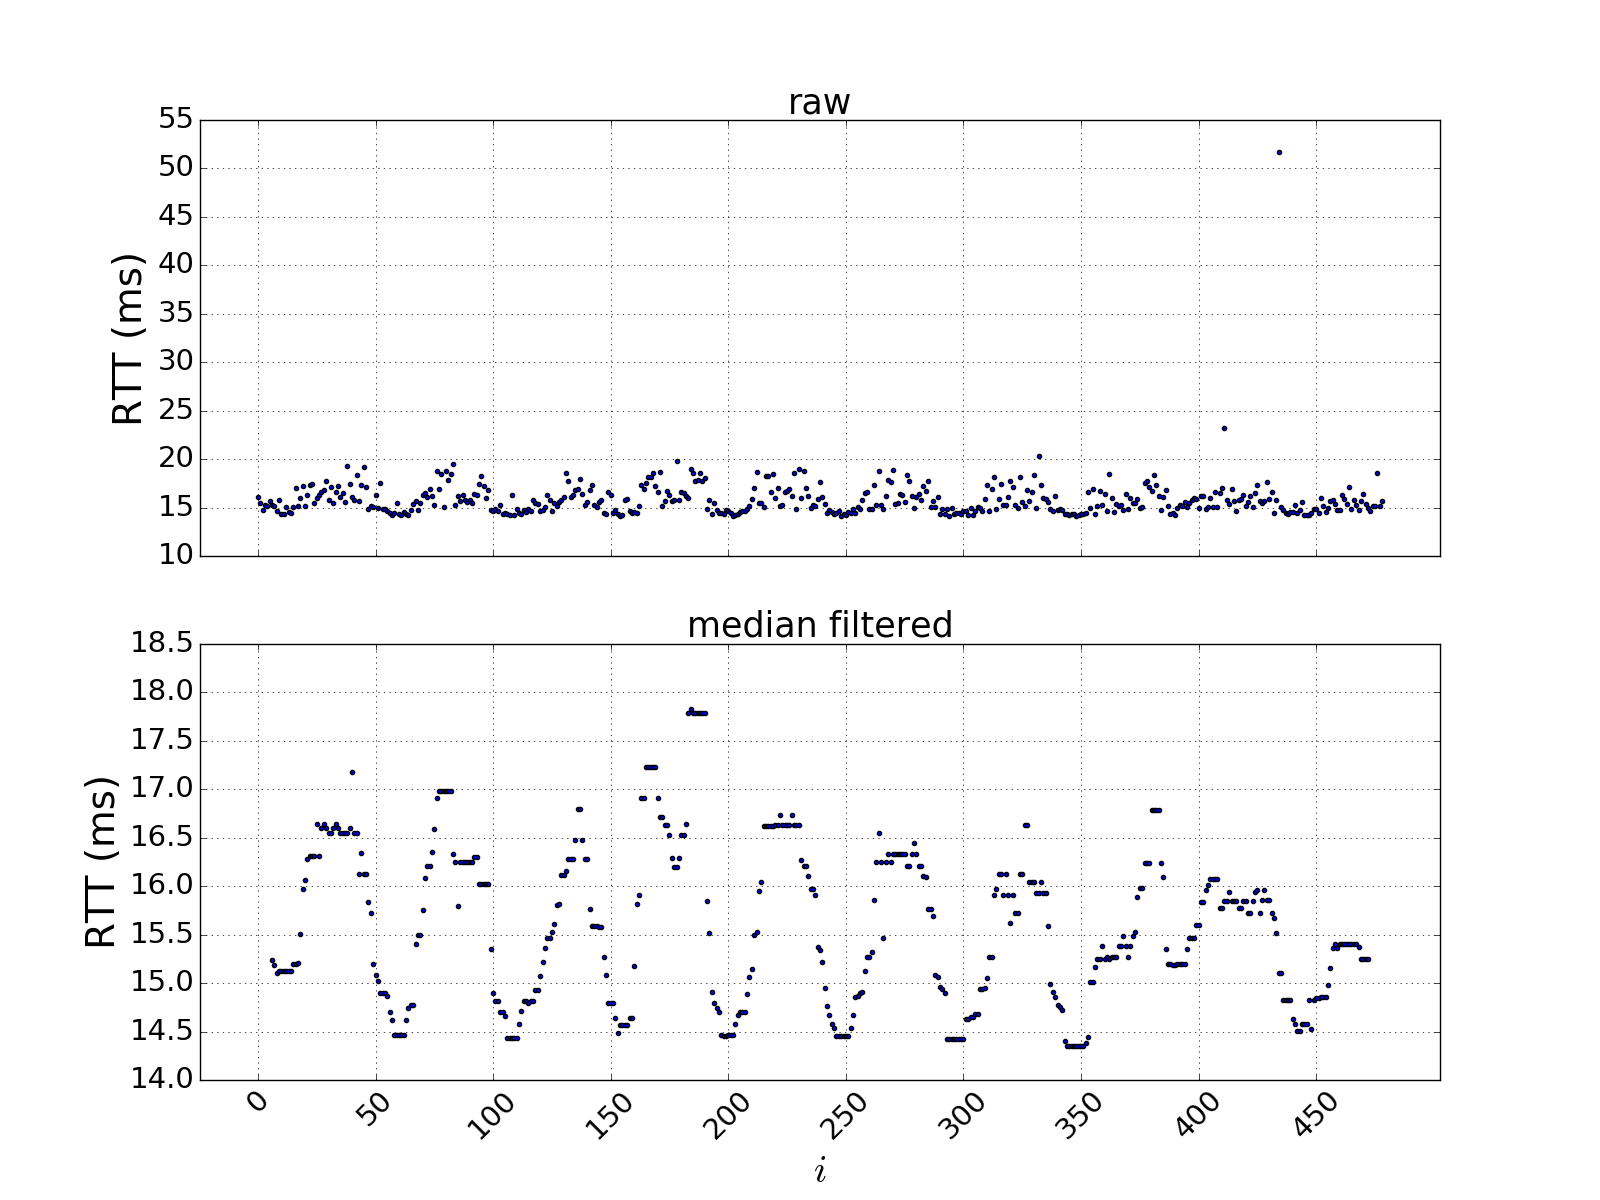
\includegraphics[width=\textwidth]{./figures/change_point_detection/preprocessing/median_filter_latency/serverAMRDTCPEV01_mac64:66:B3:4F:EC:6C_dtstart2016-07-01_dtend2016-07-11.png}
            \caption{}
        \end{subfigure}
        \begin{subfigure}[b]{0.6\textwidth}
            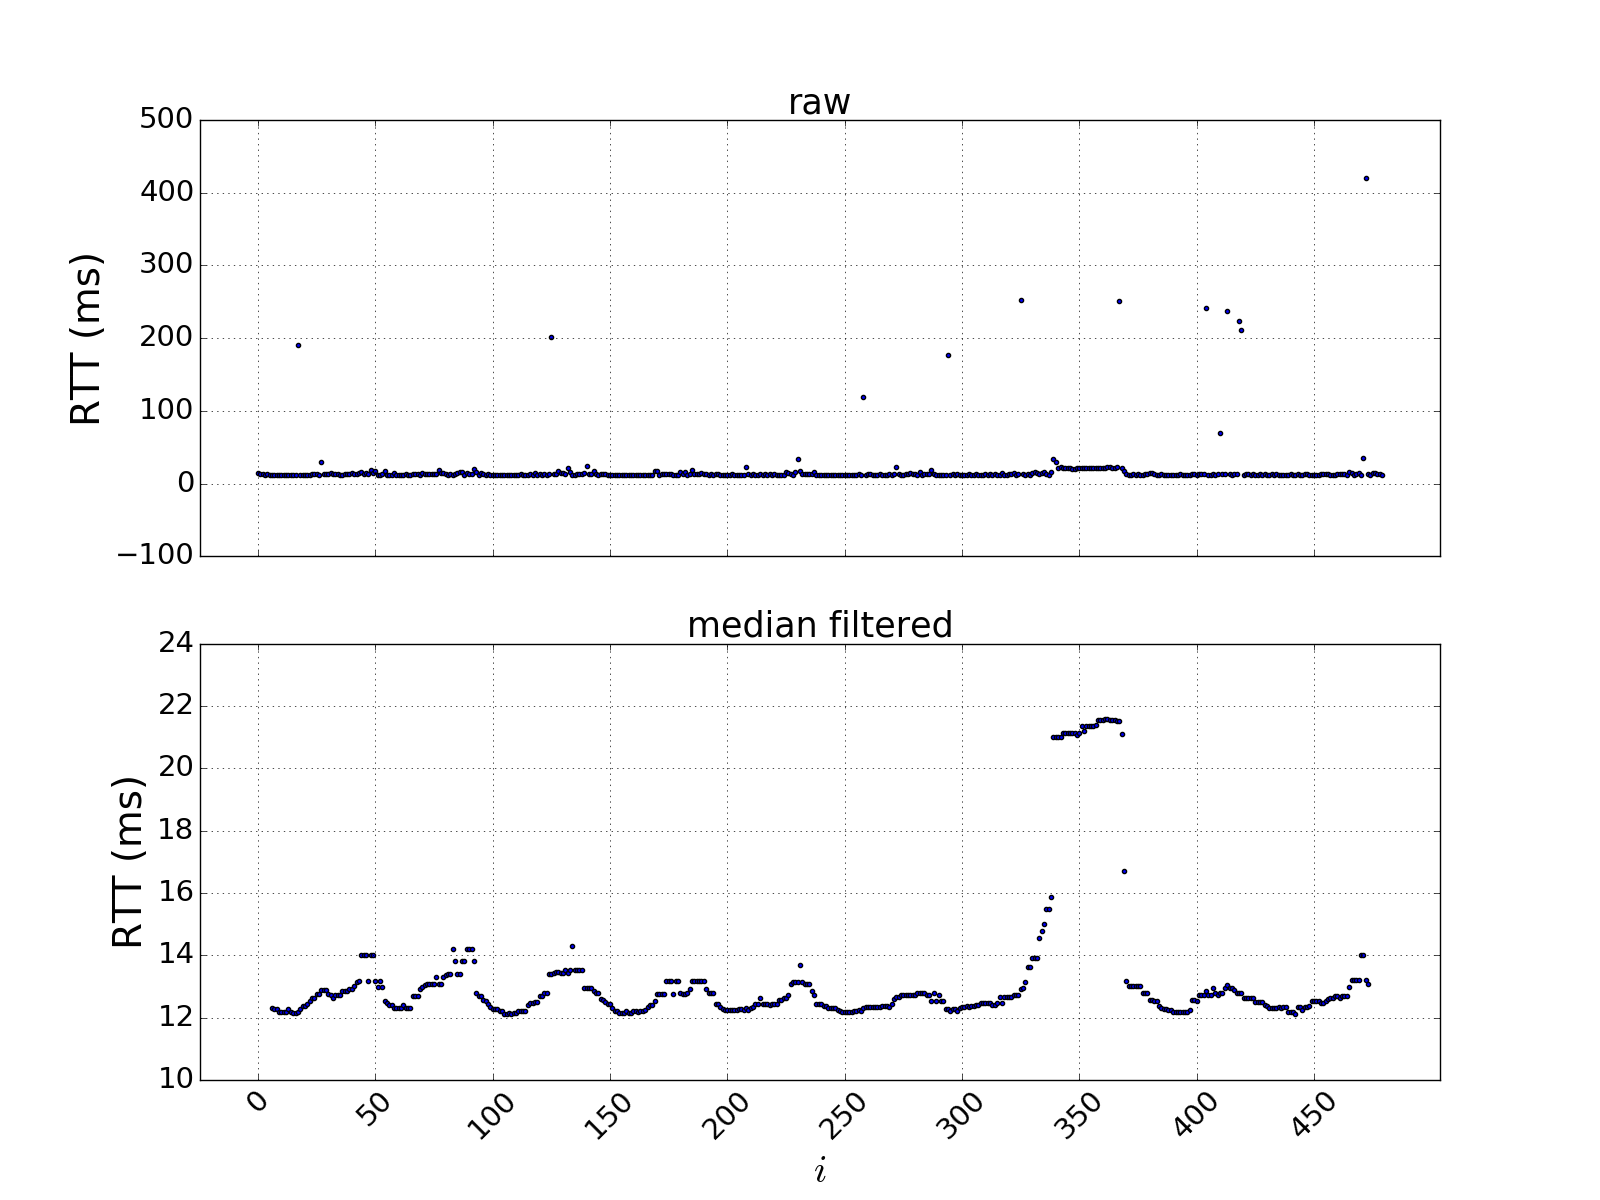
\includegraphics[width=\textwidth]{./figures/change_point_detection/preprocessing/median_filter_latency/serverAMRDTCPEV01_mac64:66:B3:4F:FD:B6_dtstart2016-07-01_dtend2016-07-11.png}
            \caption{}
        \end{subfigure}%
    }
    \caption{Median filter RTT\@. $w=6$.}
\label{fig:median_filter_rtt}
\end{figure}%

\begin{figure}[H]
    \centering
    \makebox[\textwidth][c]{%
        \begin{subfigure}[b]{0.6\textwidth}
            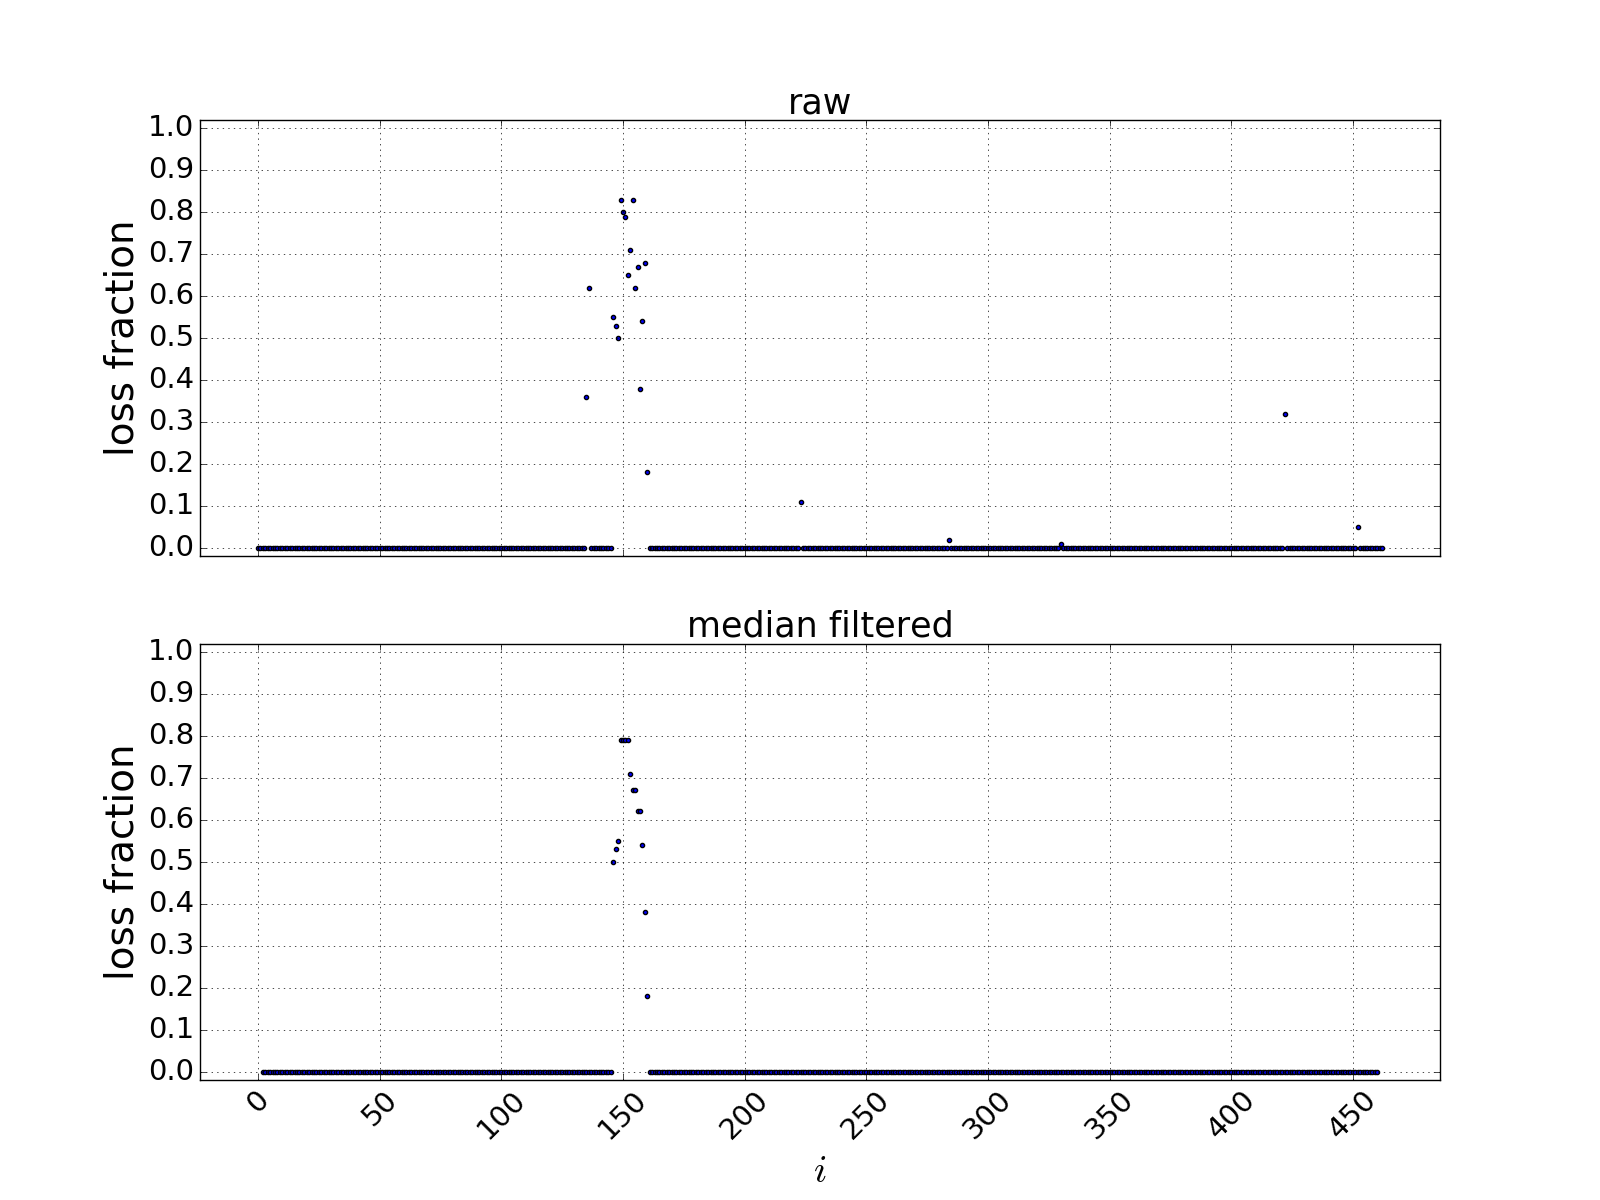
\includegraphics[width=\textwidth]{./figures/change_point_detection/preprocessing/median_filter_loss/serverAMRDTCPEV01_mac64:66:B3:4F:EB:D6_dtstart2016-07-01_dtend2016-07-11.png}
            \caption{}
        \end{subfigure}
        \begin{subfigure}[b]{0.6\textwidth}
            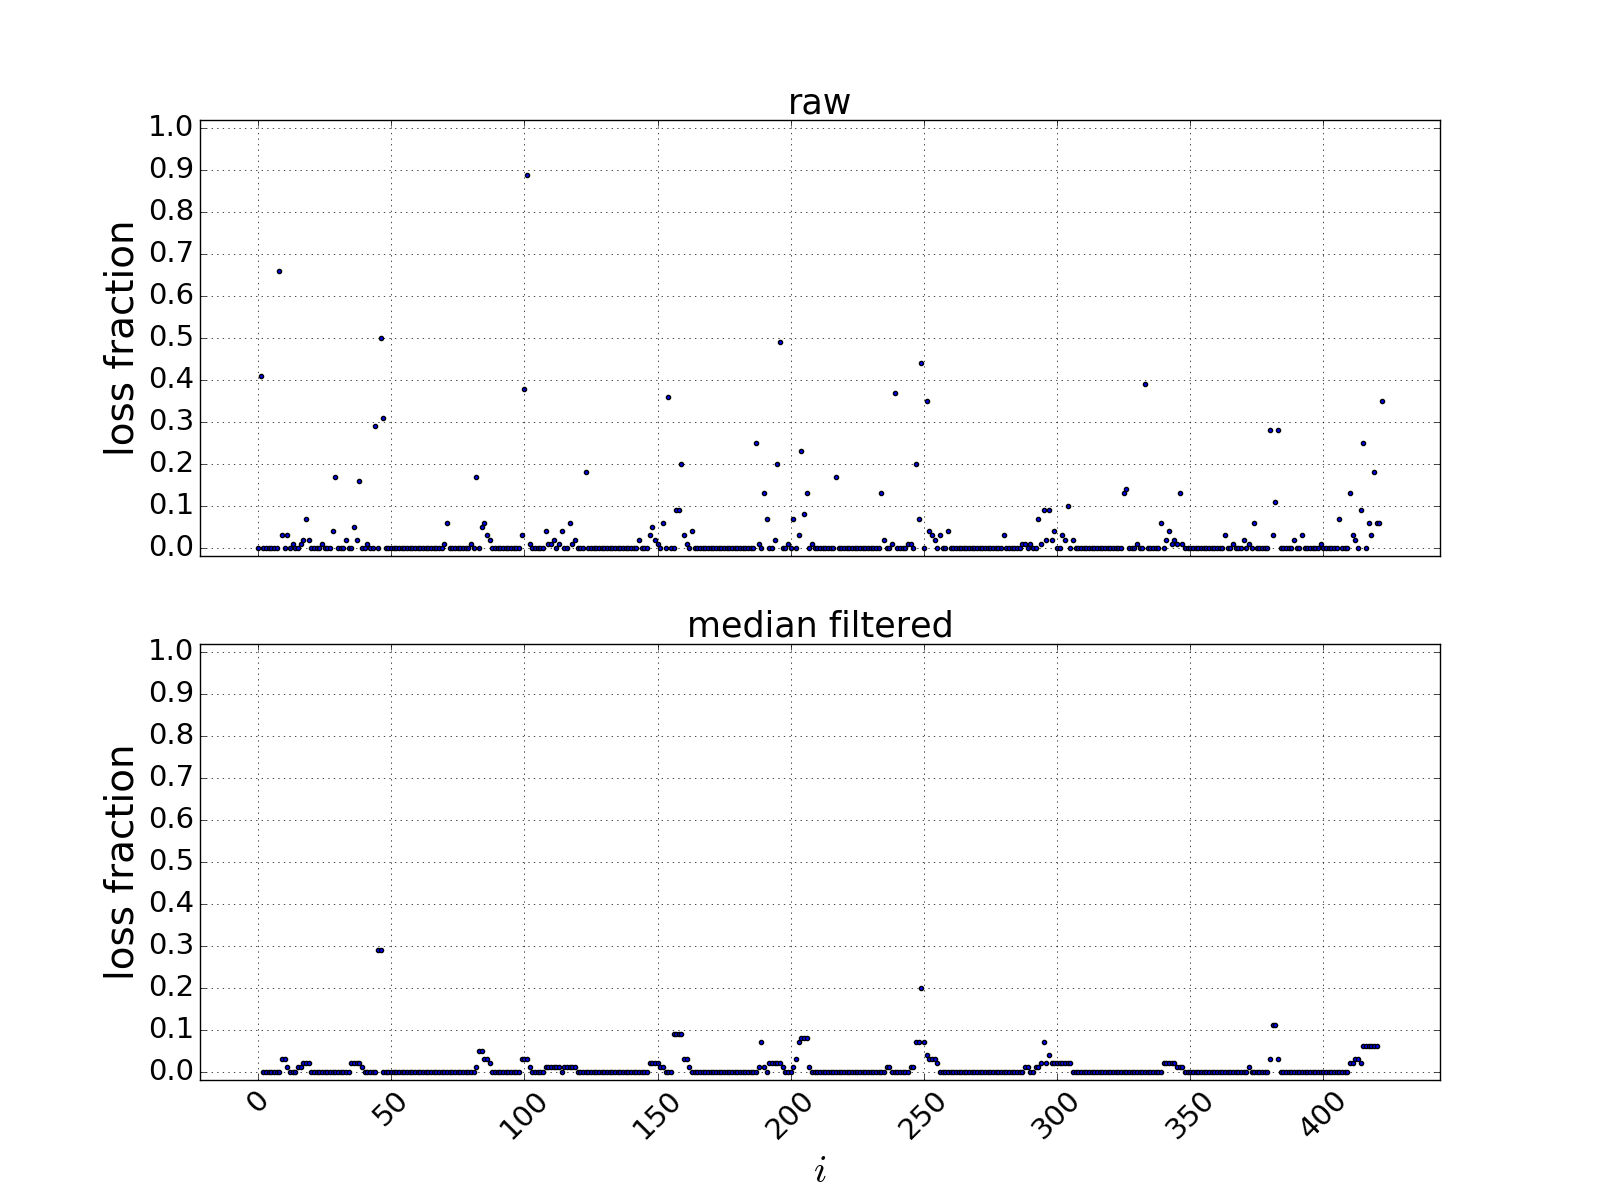
\includegraphics[width=\textwidth]{./figures/change_point_detection/preprocessing/median_filter_loss/serverAMRDTCPEV01_mac64:66:B3:4F:FE:D4_dtstart2016-07-01_dtend2016-07-11.png}
            \caption{}
        \end{subfigure}%
    }
    \caption{Median filter loss fraction. $w=2$.}
\label{fig:median_filter_loss}
\end{figure}%

\section{Sliding Windows}

Sliding windows techniques use two sliding windows over the time series, and
reduce the problem of detecting change points to the problem of testing whether
data from the segments were generated by different distributions. One approach
is to consider a distance metric between two empirical distributions as the base
to infer the change points. Letting $d(\mathbf{a}, \mathbf{b})$ be the distance
between two empirical distributions defined by the windows $\mathbf{a}$ and
$\mathbf{b}$, and considering windows of length $m$, the
Algorithm~\ref{alg:sliding_windows} presents a simple online sliding windows
method.

\begin{algorithm}[H]
\caption{Online Sliding Windows}
\label{alg:sliding_windows}
    \begin{algorithmic}[1]
        \State{} $i \gets 1$
        \While{$i + 2 m - 1 \leq n$}
             \If{$d(\mathbf{y}_{i : i + m - 1}, \mathbf{y}_{i + m : i + 2m - 1}) > \alpha$}
                \State{} Report $i + m - 1$ as a change point
                \State{} $i \gets i + m$
             \Else{}
                \State{} $i \gets i + 1$
             \EndIf{}
        \EndWhile{}
    \end{algorithmic}
\end{algorithm}

The distance
function has a direct impact on the classification accuracy.
Therefore, several
distance measures where tested, such as mean difference, relative mean
difference,
Hellinger~\cite{hellinger_distance}, Kolmogorov-Smirnov, and
Earth Mover's
Distance~\cite{the_earth_movers_distance_as_a_metric_for_image_retrieval}.

Figure~\ref{fig:sliding_windows_online} is an example of the online sliding
windows execution. The top plot
shows the RTT over time, and in
the bottom plot, the $(i, D_{i})$ point represents the distance between
$\mathbf{y}_{i - m : i - 1}$ and $\mathbf{y}_{i : i + m - 1}$. The red vertical
line indicates a detected change point, and the green horizontal line
illustrates the used threshold.

\begin{figure}[H]
    \centering
    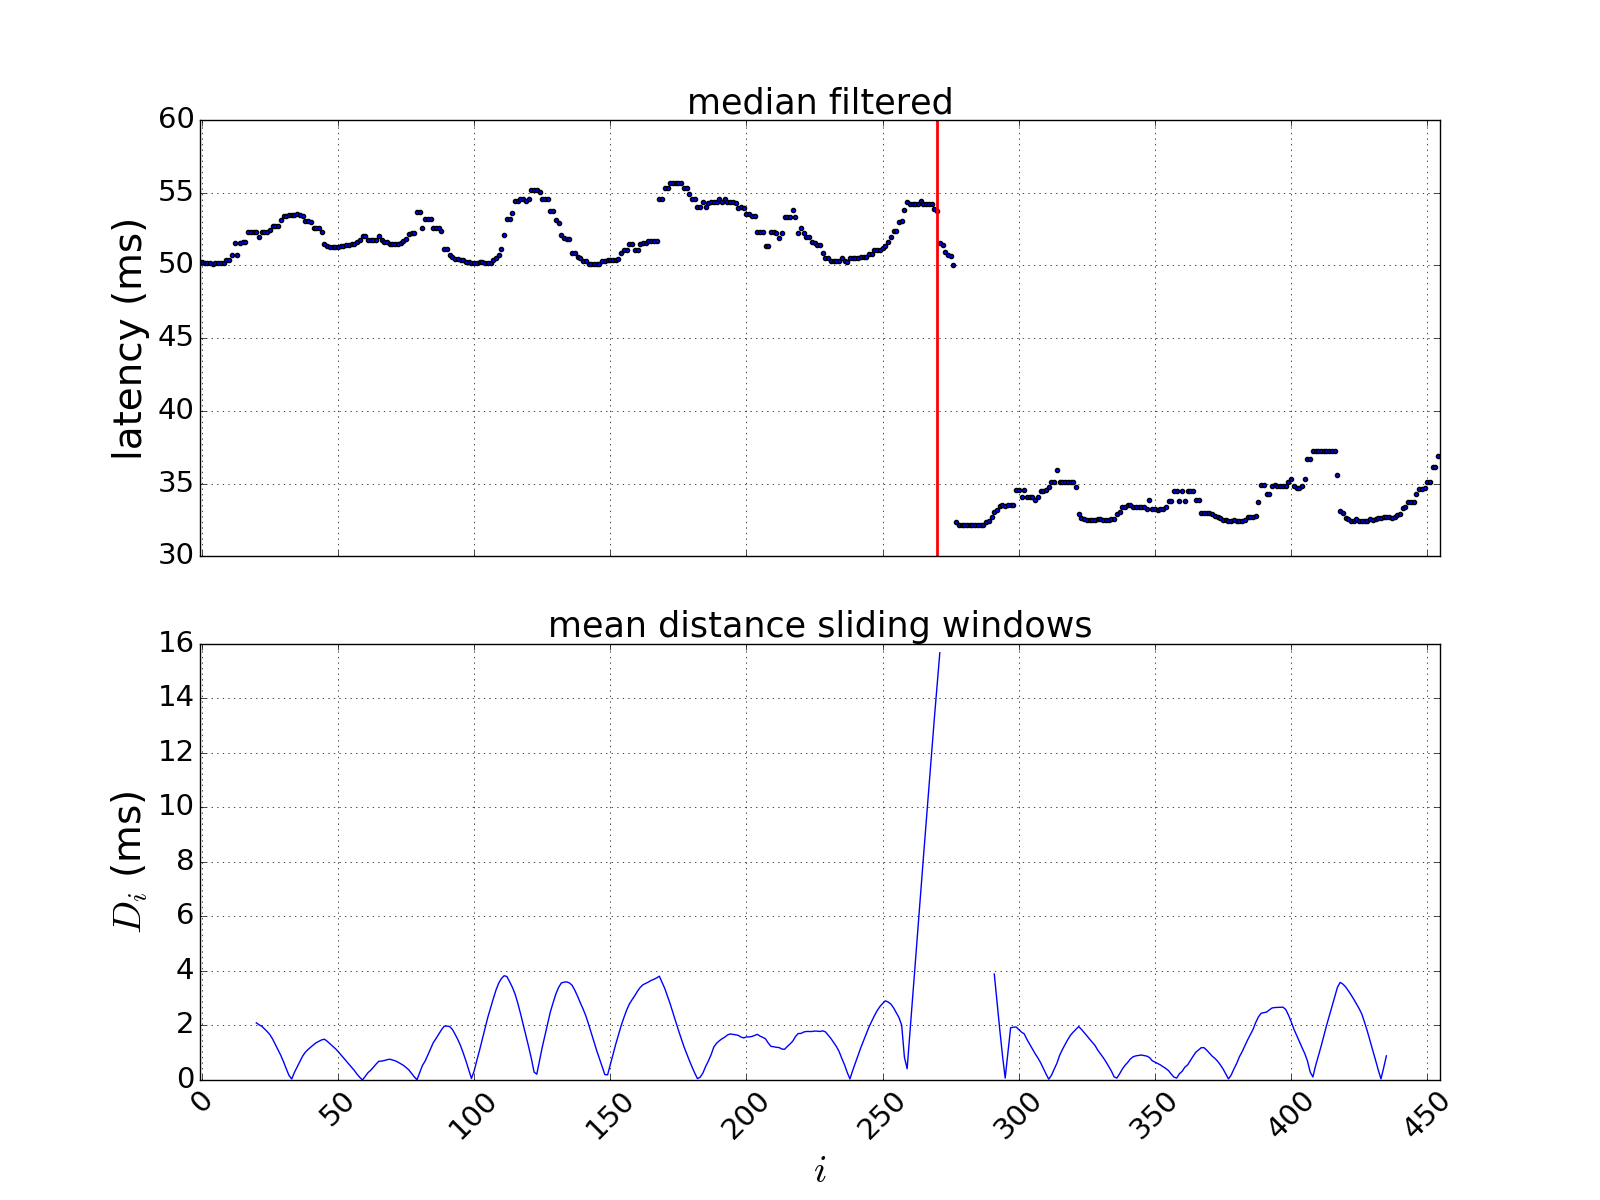
\includegraphics[width=0.7\textwidth]{./figures/change_point_detection/sliding_windows_online/id100_serverNHODTCSRV04_mac64:66:B3:A6:B3:22_dtstart2016-07-01_dtend2016-07-11.png}
    \caption{Online Sliding Windows.}
\label{fig:sliding_windows_online}
\end{figure}%

It is possible to note that the detected change point is on the left of the
correct location.
This occurred since the distance between the windows was still
increasing when reached the threshold. Therefore, for the offline
version, it was defined that a peak detection method is applied on
the sliding windows distance time series.
An execution example is found in
Figure~\ref{fig:sliding_windows_offline}.

\begin{figure}[H]
    \centering
    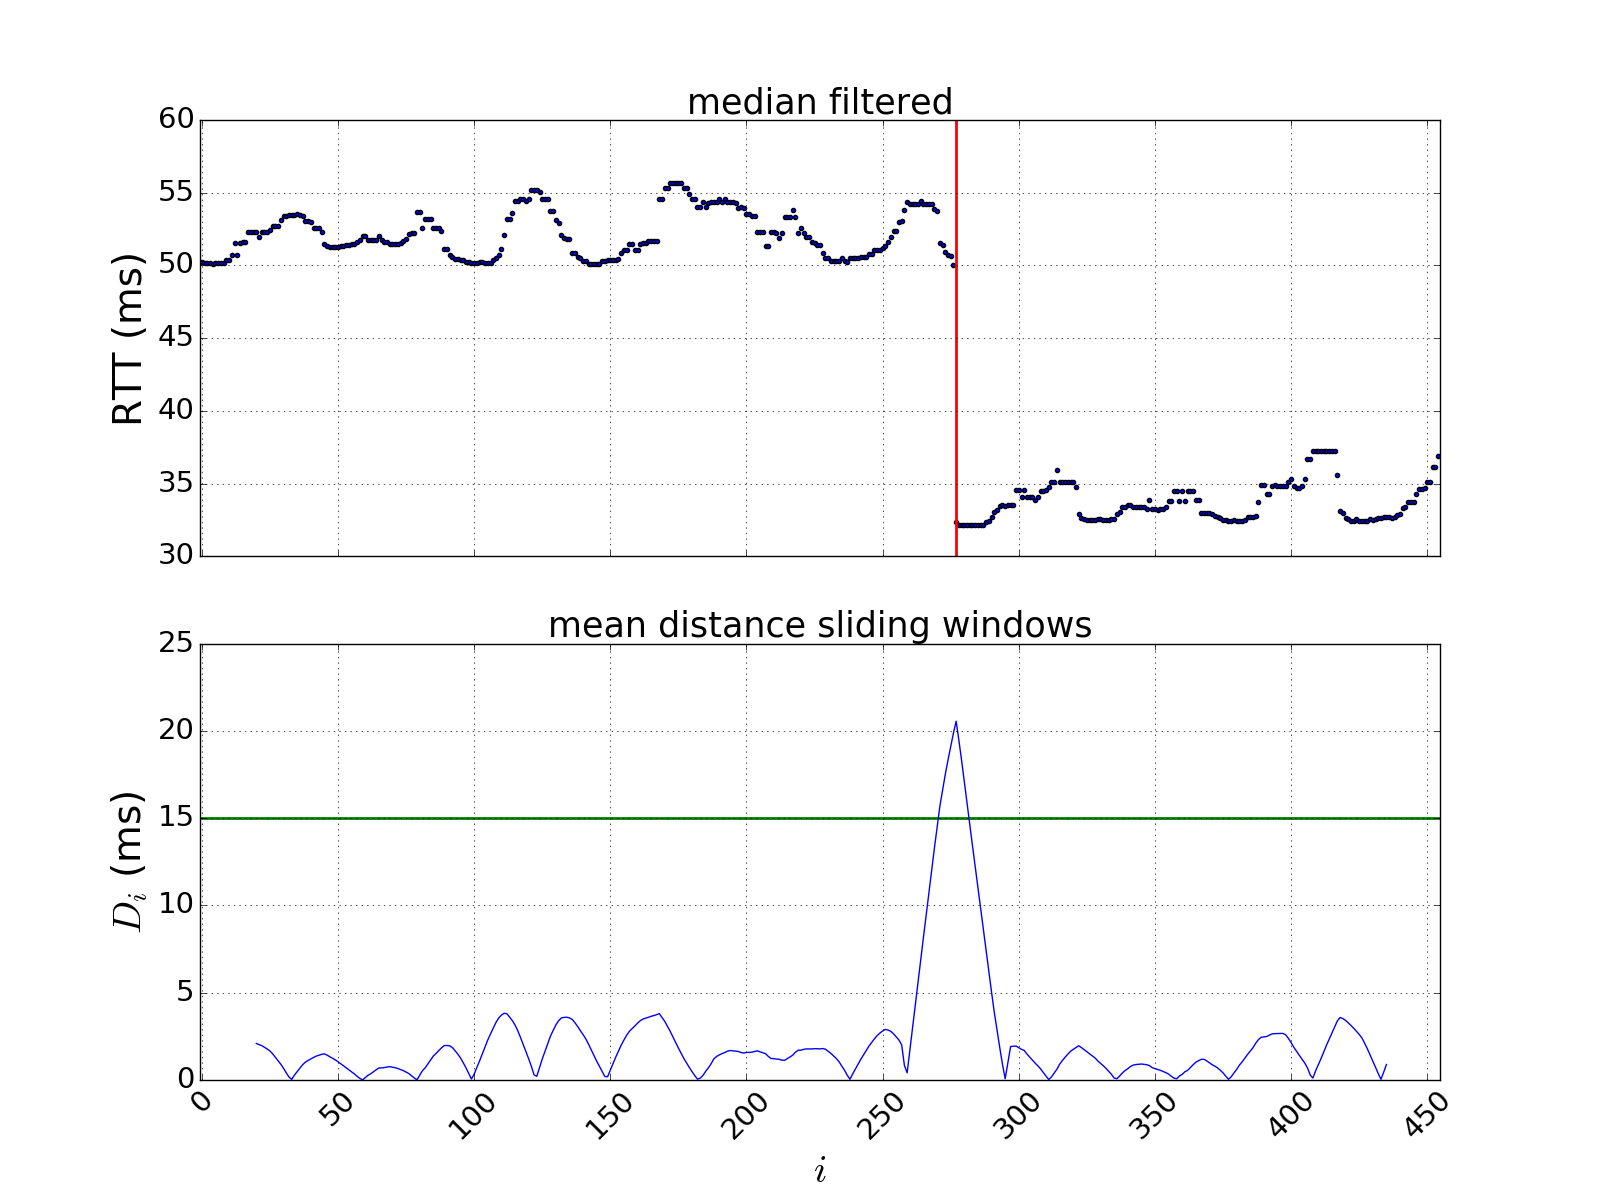
\includegraphics[width=0.7\textwidth]{./figures/change_point_detection/sliding_windows_offline/id100_serverNHODTCSRV04_mac64:66:B3:A6:B3:22_dtstart2016-07-01_dtend2016-07-11.png}
    \caption{Offline Sliding Windows.}
\label{fig:sliding_windows_offline}
\end{figure}%

As stated in~\cite{detecting_change_in_data_streams}, a performance improvement
can be achieved concurrently executing the same sliding windows algorithm with
different windows lengths. This change facilitates the detection of
segments with distinct number of points.

\section{Optimization Model}

Given a fixed value of $k$, one approach is to define a cost function that
measures the homogeneity of a window, and therefore, choose the change points
that globally optimize this homogeneity. Let the cost of the $i$-th segment be
defined as $C(\mathbf{y}_{\tau_{i - 1} + 1 : \tau_{i}})$, then the cost of a
segmentation is the sum of all segments costs.

A common choice for the function $C$ is the MSE (Mean Squared Error), which can
capture changes in the mean. Another usual approach is to consider distribution
changes through negative maximum log-likelihood functions, considering that data
within a window is iid.

Therefore, given a fixed $k$, the optimal segmentation is obtained through the
following optimization problem, which is called the constrained
case~\cite{on_optimal_multiple_changepoint_algorithms_for_large_data}:

\begin{equation}
    \min_{\boldsymbol \tau_{1 : k}} \sum \limits_{i = 1}^{k + 1} C(\mathbf{y}_{\tau_{i - 1} + 1 : \tau_{i}})
\end{equation}

This problem can be solved using dynamic programming with $O(k n^2 f(n))$ time
complexity, where $f(n)$ is related with the cost function evaluation. Several
segment cost functions can be evaluated in $O(1)$ after a $O(n)$ preprocessing
phase, implying in an overall $O(k n^2)$ complexity. It is possible to prove
that MSE, negative maximum log-likelihood functions of normal, exponential,
poisson and binomial distributions have this characteristic. Also, the
formulation can consider a minimum value of a window length.

Modeling segments with distributions can lead to practical difficulties. One of
them is the fact that segments can form degenerate distributions, that is, the
data of a window can have zero variance, which is always the case of unitary
length windows. In these scenarios the negative maximum log-likelihood can be
undefined. Despite this issue has not been described in the literature,
this work followed two approaches to overcome this situation. The first one
tries to avoid degenerate segments adding a white noise with small variance to
the data stream. The second one considers that the cost of any degenerate
distribution is equal to a constant.

When the number of change points is unknown, an usual way is to introduce a non
decreasing penalty function $g(k)$. Then, the new optimization problem, called
penalized case~\cite{on_optimal_multiple_changepoint_algorithms_for_large_data},
is:

\begin{equation}
    \min_{k, \boldsymbol \tau_{1 : k}} \sum \limits_{i = 1}^{k + 1} C(\mathbf{y}_{\tau_{i - 1} + 1 : \tau_{i}}) + g(k)
\end{equation}

This problem can be solved in $O(K n^{2} f(n))$. However, if the penalty
function is linear in $k$, the problem can be formulated more efficiently and
solved in $O(n^{2} f(n))$.

Also, there are several pruning algorithms to speedup the
computation~\cite{optimal_detection_of_changepoints_with_a_linear_computational_cost, on_optimal_multiple_changepoint_algorithms_for_large_data, computationally_efficient_changepoint_detection_for_a_range_of_penalties},
in general trying to reduce the $\boldsymbol \tau$ search space but maintaining
optimality.

When a negative maximum log-likelihood is
used, the cost of a segment with an outlier can be orders of magnitude greater
than the cost of a window without anomalies. Therefore,
in this case, the method is sensible to outliers.

Figure~\ref{fig:seg_neigh} presents two output examples.

\begin{figure}[H]
    \centering
    \makebox[\textwidth][c]{%
        \begin{subfigure}[b]{0.5\textwidth}
            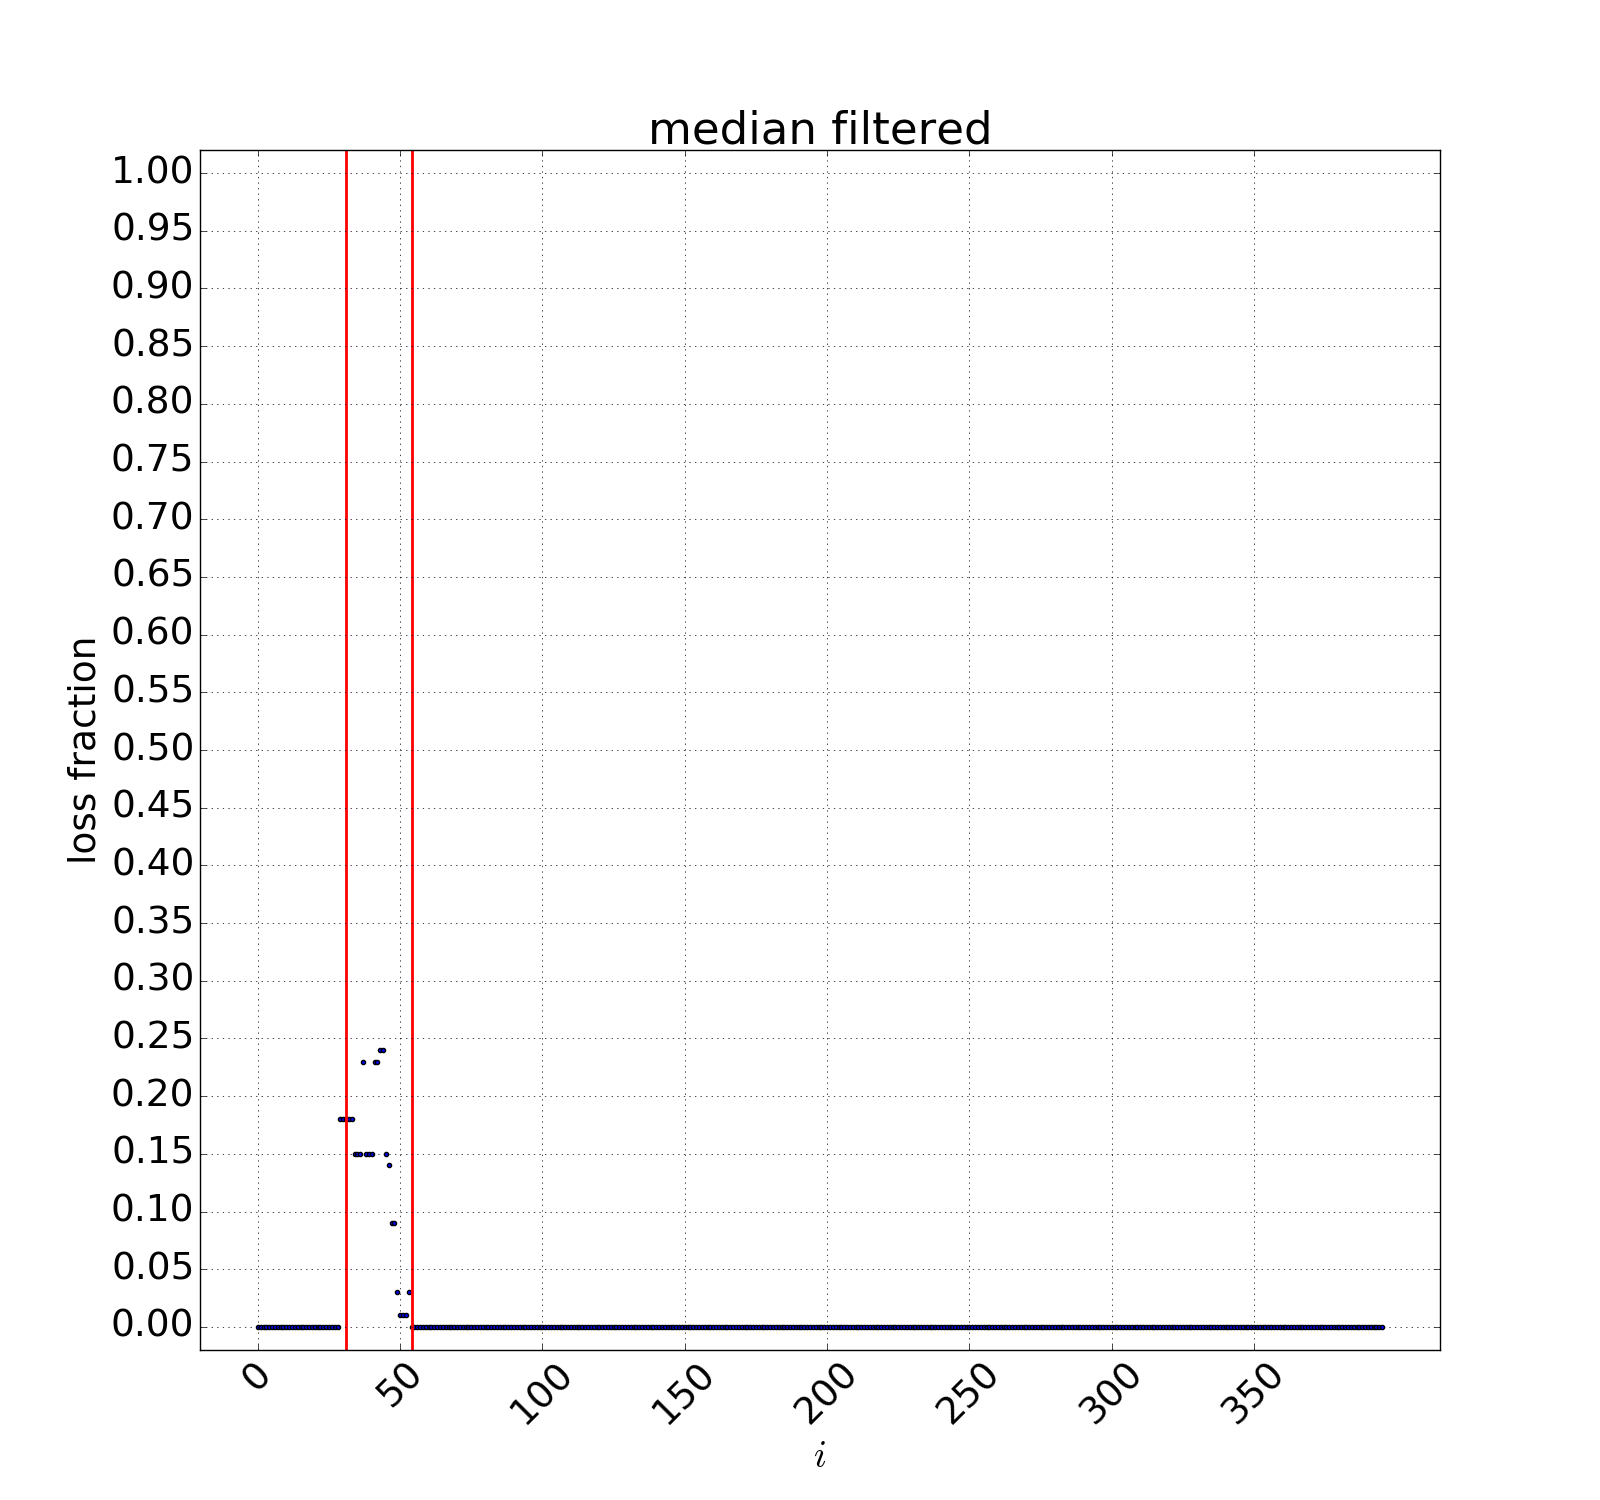
\includegraphics[width=\textwidth]{./figures/change_point_detection/seg_neigh/id7_serverRIBDTCSRV03_mac64:66:B3:A6:BB:10_dtstart2016-07-01_dtend2016-07-11.png}
            \caption{}
        \end{subfigure}
        \begin{subfigure}[b]{0.5\textwidth}
            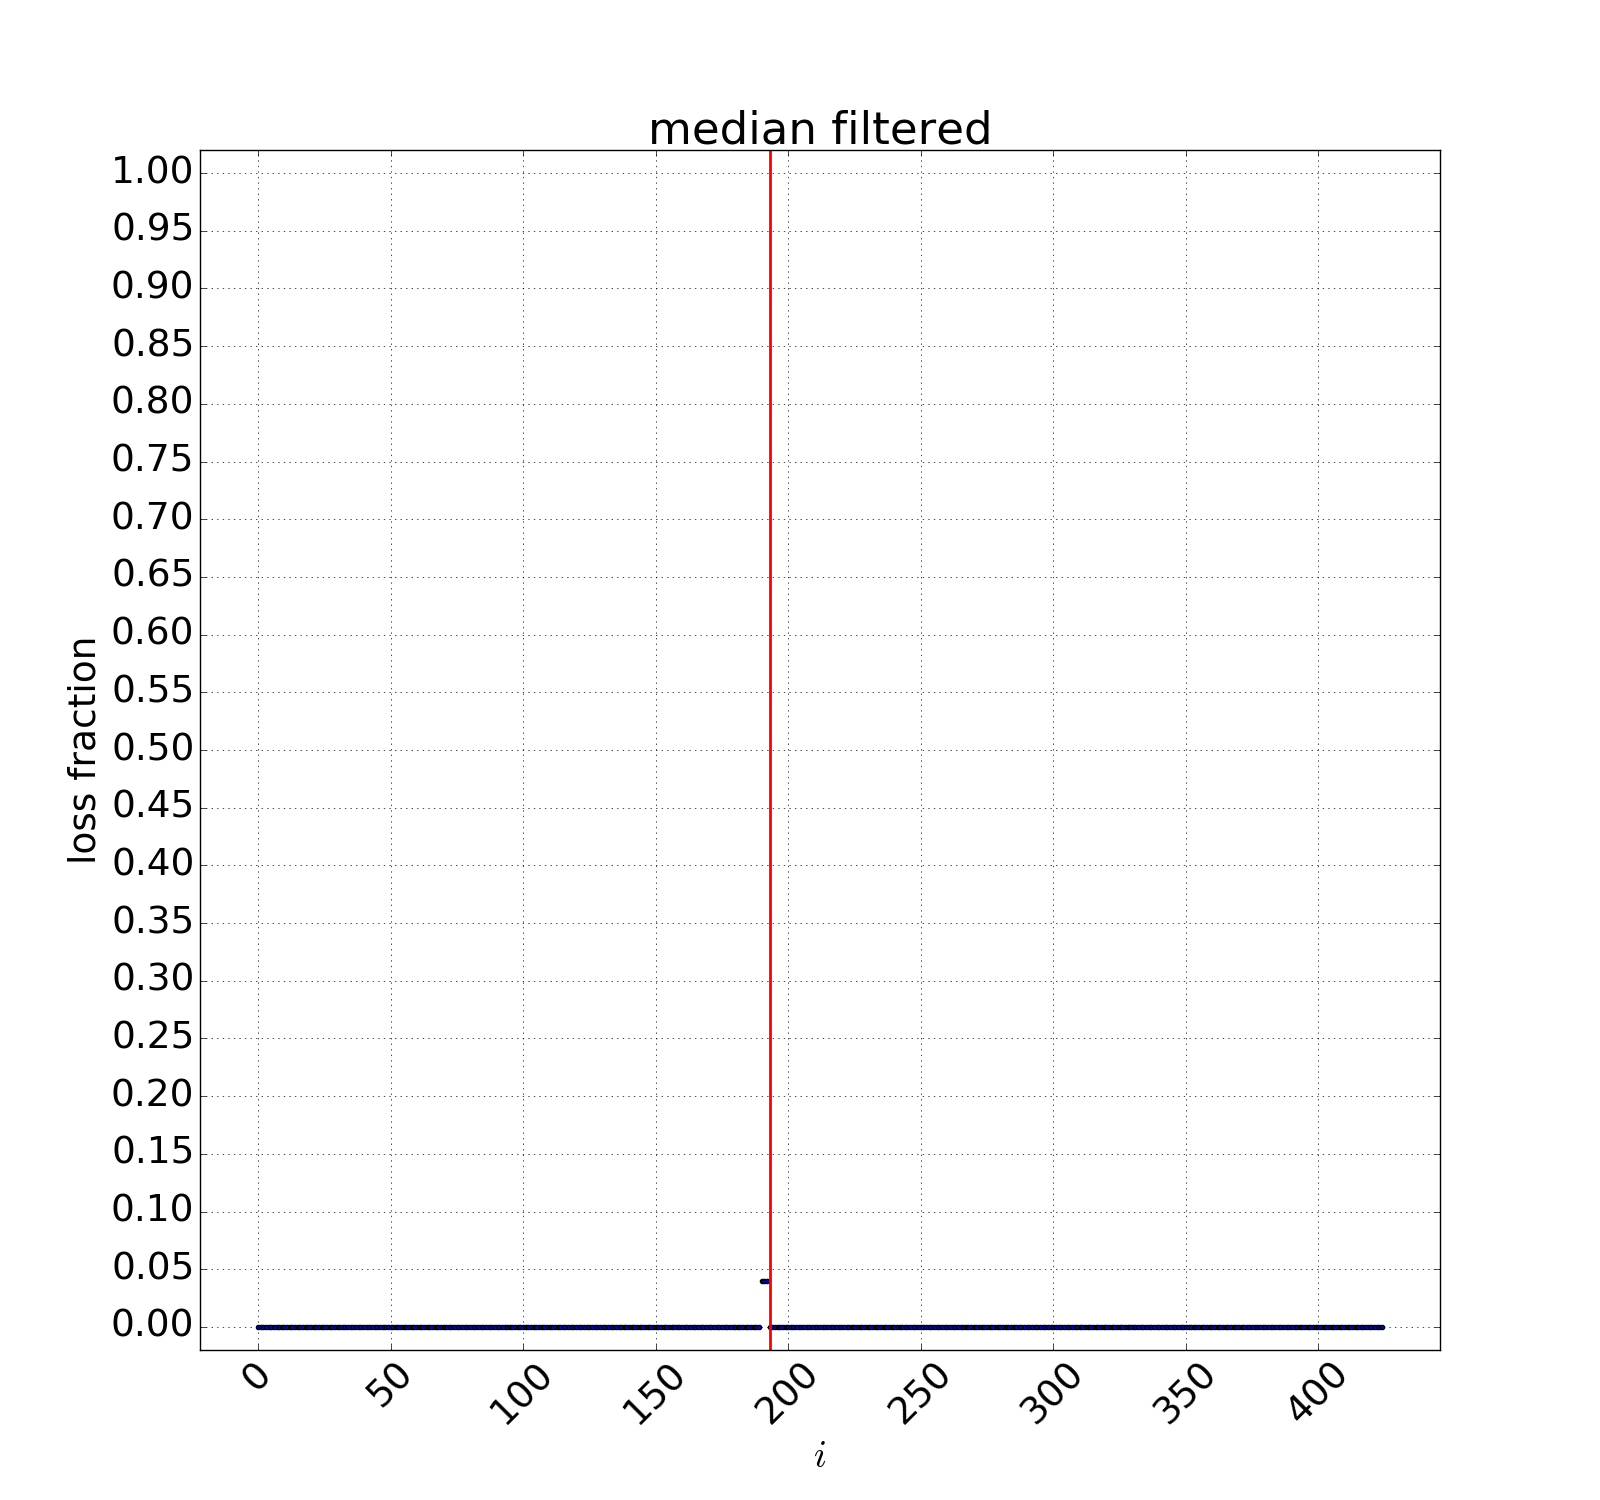
\includegraphics[width=\textwidth]{./figures/change_point_detection/seg_neigh/id158_serverSOCDTCPEV01_mac64:66:B3:A6:B9:D2_dtstart2016-07-01_dtend2016-07-11.png}
            \caption{}
        \end{subfigure}%
    }
    \caption{Optimization model.}
\label{fig:seg_neigh}
\end{figure}%

\section{HMM (Hidden Markov Model)}

The idea that each segment is associated with a specific latent configuration
has a direct interpretation to a HMM
model~\cite{a_hidden_markov_model_segmentation_procedure_for_hydrological_and_environmental_time_series, fast_estimation_of_posterior_probabilities_in_change-point_analysis_through_a_constrained_hidden_markov_model, inertial_hidden_markov_models_modeling_change_in_multivariate_time_series}.
In this context, each window is related to a hidden state of a HMM, and the
observation distribution of this state represents the distribution of that
segment. Therefore, the mechanism models the time series using a HMM, and
through the hidden state path, assesses the times when a transition between
different hidden states occur.

There are several approaches in the detection and training phases. For example,
given a trained HMM, the most probable hidden state path can be checked through
the Viterbi algorithm. Also, it is possible to evaluate the probability of a
transition between different hidden states at time $t$, and then apply a
threshold and peak detection methods, as well as in sliding windows techniques.
For the training step, it is possible to use several time series to train a
single HMM, and then use this model to detect change points in all time series.
Another way is to, for each data stream, train a single model using only the
target time series.

It is important to note that the structure of the hidden state graph has a large
impact on the performance. Using a fully connected graph, the number of states
defines the maximum number of distribution configurations. Employing a left to
right structure, the number of hidden states will impact the maximum number of
segments.

In~\cite{inertial_hidden_markov_models_modeling_change_in_multivariate_time_series}
is stated that when using a fully connected structure, the time interval that a
time series stays in the same hidden state is low, which can not reflect real
data. To overcome this problem,
\cite{inertial_hidden_markov_models_modeling_change_in_multivariate_time_series}
suggests to increase the time that a time series stands in the same hidden
state using a dirichlet prior regularization. However, it was empirically
verified that it is difficult to choose good parameters for this strategy.
Instead, to surpass this issue,
when using the best hidden state path, this dissertation used a HMM only as a
filter, which acts as a dimensional reduction that takes into consideration
temporal
patterns. In this scenario, the best hidden state sequence is the input to
a sliding windows method with a discrete Hellinger distance.

Figure~\ref{fig:hmm_filter} presents an execution using a fully connected HMM
with observations following a Normal distribution.
The top plot is the median filtered time series.
The middle plot is the best hidden state path, in which the vertical axis
indicates the distribution of each hidden state.
The bottom plot is the sliding windows distance.

\begin{figure}[H]
    \centering
    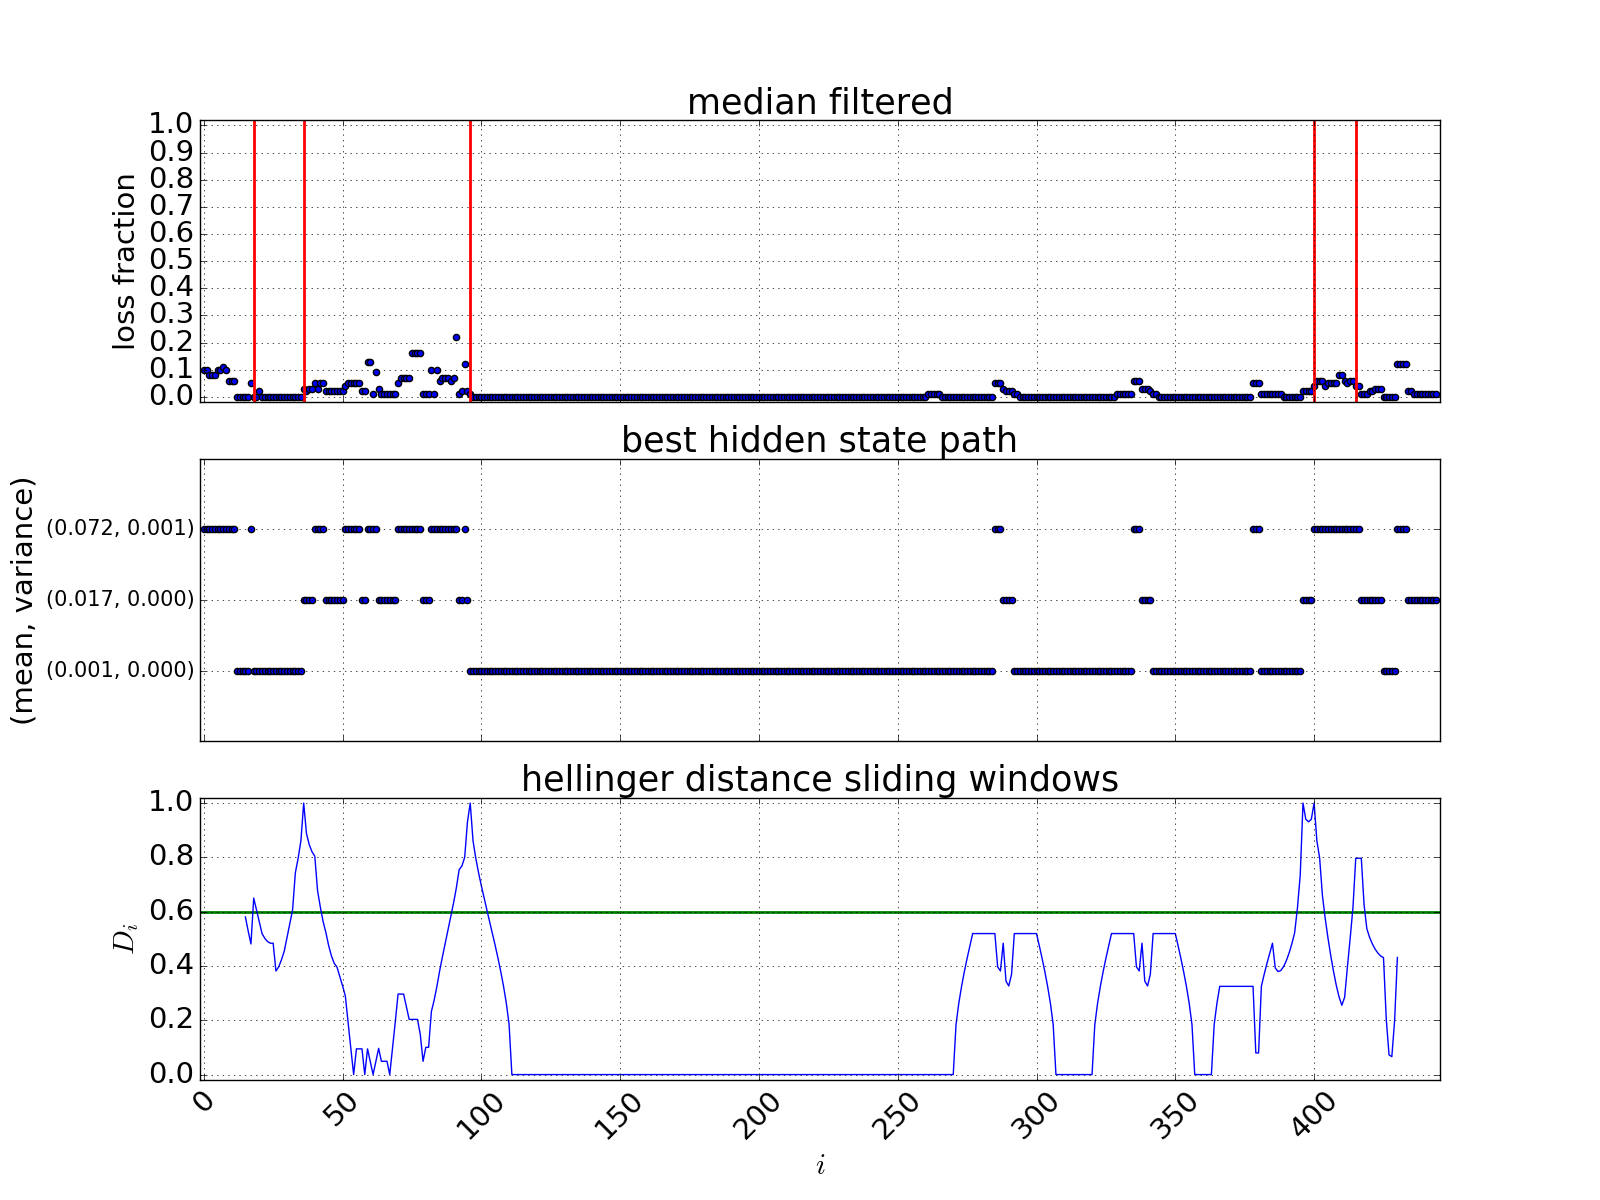
\includegraphics[width=0.8\textwidth]{./figures/change_point_detection/gaussian_hmm/id115_serverRJODTCLDM031_mac64:66:B3:7B:A1:B8_dtstart2016-05-01_dtend2016-05-11.png}
    \caption{HMM filter.}
\label{fig:hmm_filter}
\end{figure}%

\section{Bayesian Inference}

There are several Bayesian methods which aims to assess the probability that a
point is a change point. Following an offline fashion, the work
of~\cite{exact_and_efficient_bayesian_inference_for_multiple_changepoint_problems}
recursively calculates, for each $i$, the probability of $\mathbf{y}_{i : n}$
given a change point at $i$. With these probabilities is possible to simulate
the time of the first change point, and then, compute the conditional
distribution of the time of the second change given the first, and so on. To
achieve this, the mechanism assumes that observations are independents, and that
each segment is modeled by conjugate priors. Also, the procedure considers
priors to model the number of changes and the time between two consecutive
change points. Depending of the priors choices, the overall complexity of this
method can be $O(n^{2})$.

In~\cite{bayesian_online_changepoint_detection} it is also considered that
parameters of different segments are independents, and that data within a
window is iid. However, through an online mode, the procedure is concerned with
the estimation of the distribution of the length of the current time since the
last change point, called run length, given the data so far observed. To achieve
this, the method assumes the probability of current run length given the last
run length as a prior. Assuming exponential-family likelihoods to model a
segment, the time complexity to process a point is linear in the number of
points already observed.

As with the previous procedures, in both cases is applied a peak detection
algorithm in the probability time series. Also,
these methods can be sensible to outliers, specially the
online version. Furthermore, it was empirically noticed that, in general, the
probabilities are only non zero around the probability peaks.
Figure~\ref{fig:bayesian_inference} illustrates the bayesian inference
algorithms executions.

\begin{figure}[H]
    \centering
    \makebox[\textwidth][c]{%
        \begin{subfigure}[b]{0.6\textwidth}
            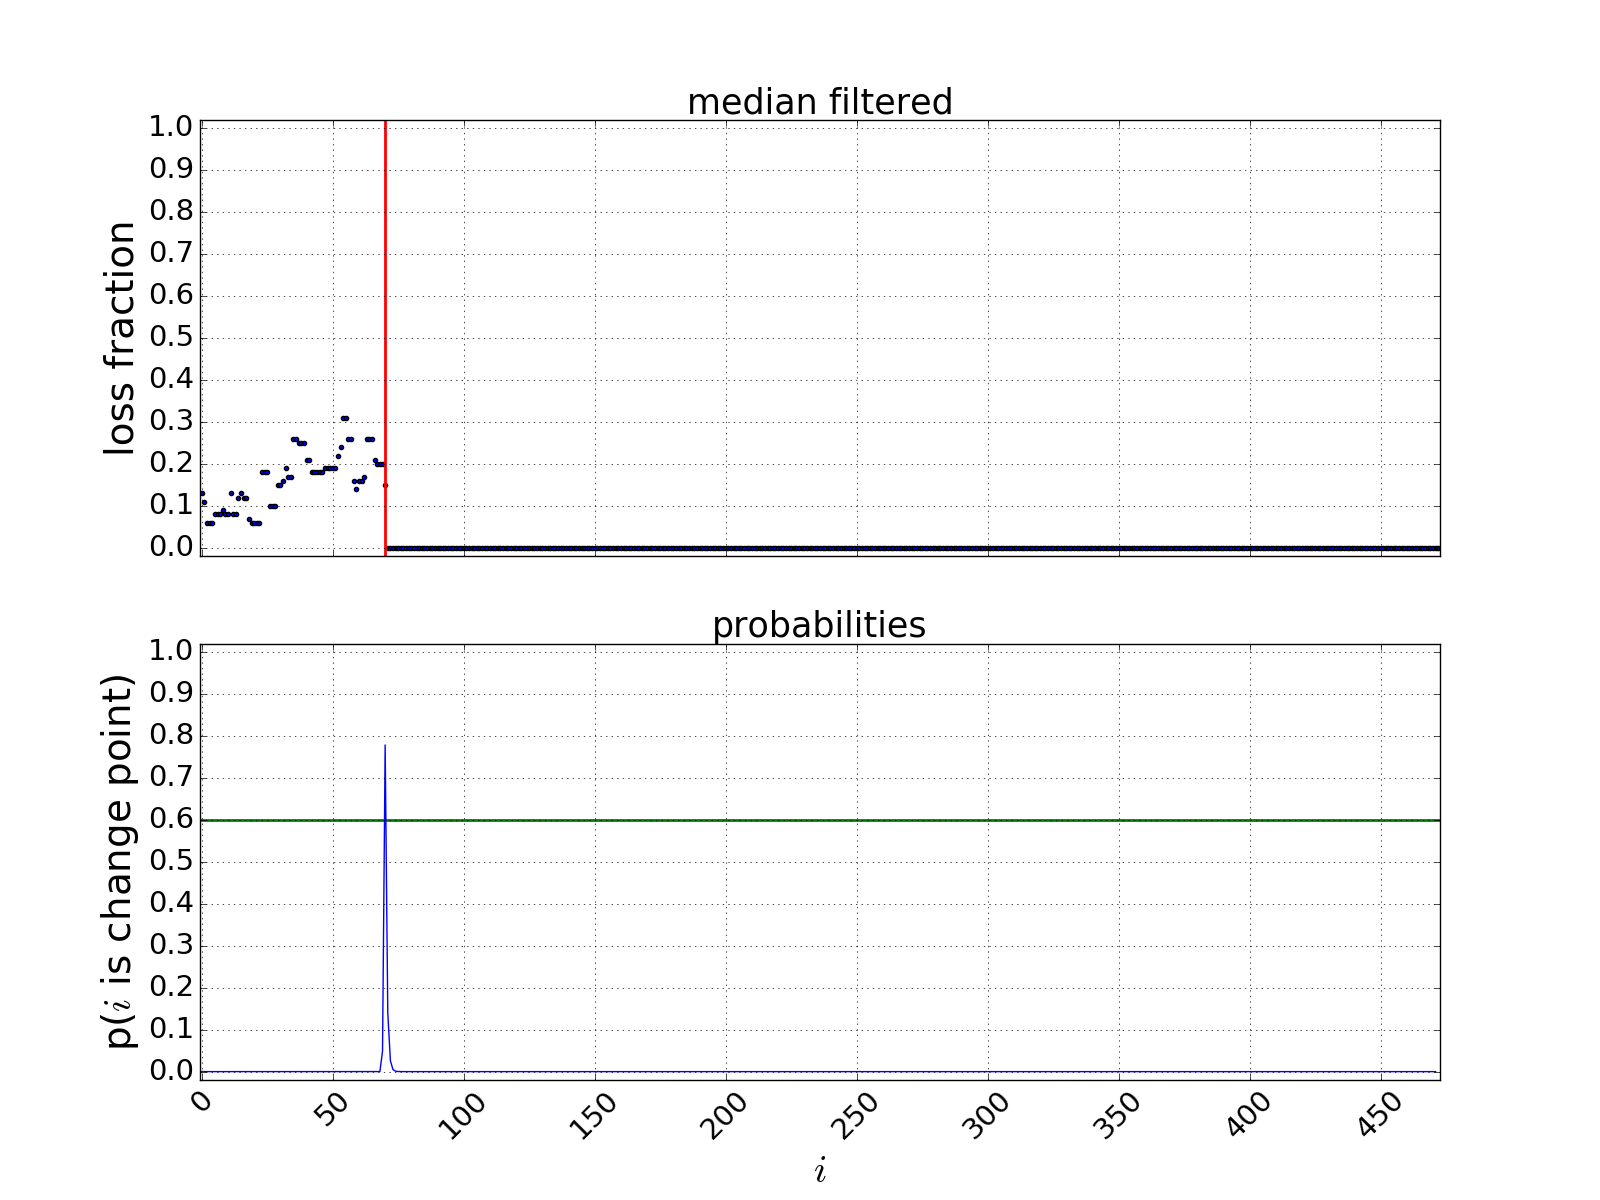
\includegraphics[width=\textwidth]{./figures/change_point_detection/bayesian_offline/id305_serverSNEDTCPROB01_mac64:66:B3:A6:BB:80_dtstart2016-07-01_dtend2016-07-11.png}
            \caption{Offline.}
        \end{subfigure}
        \begin{subfigure}[b]{0.6\textwidth}
            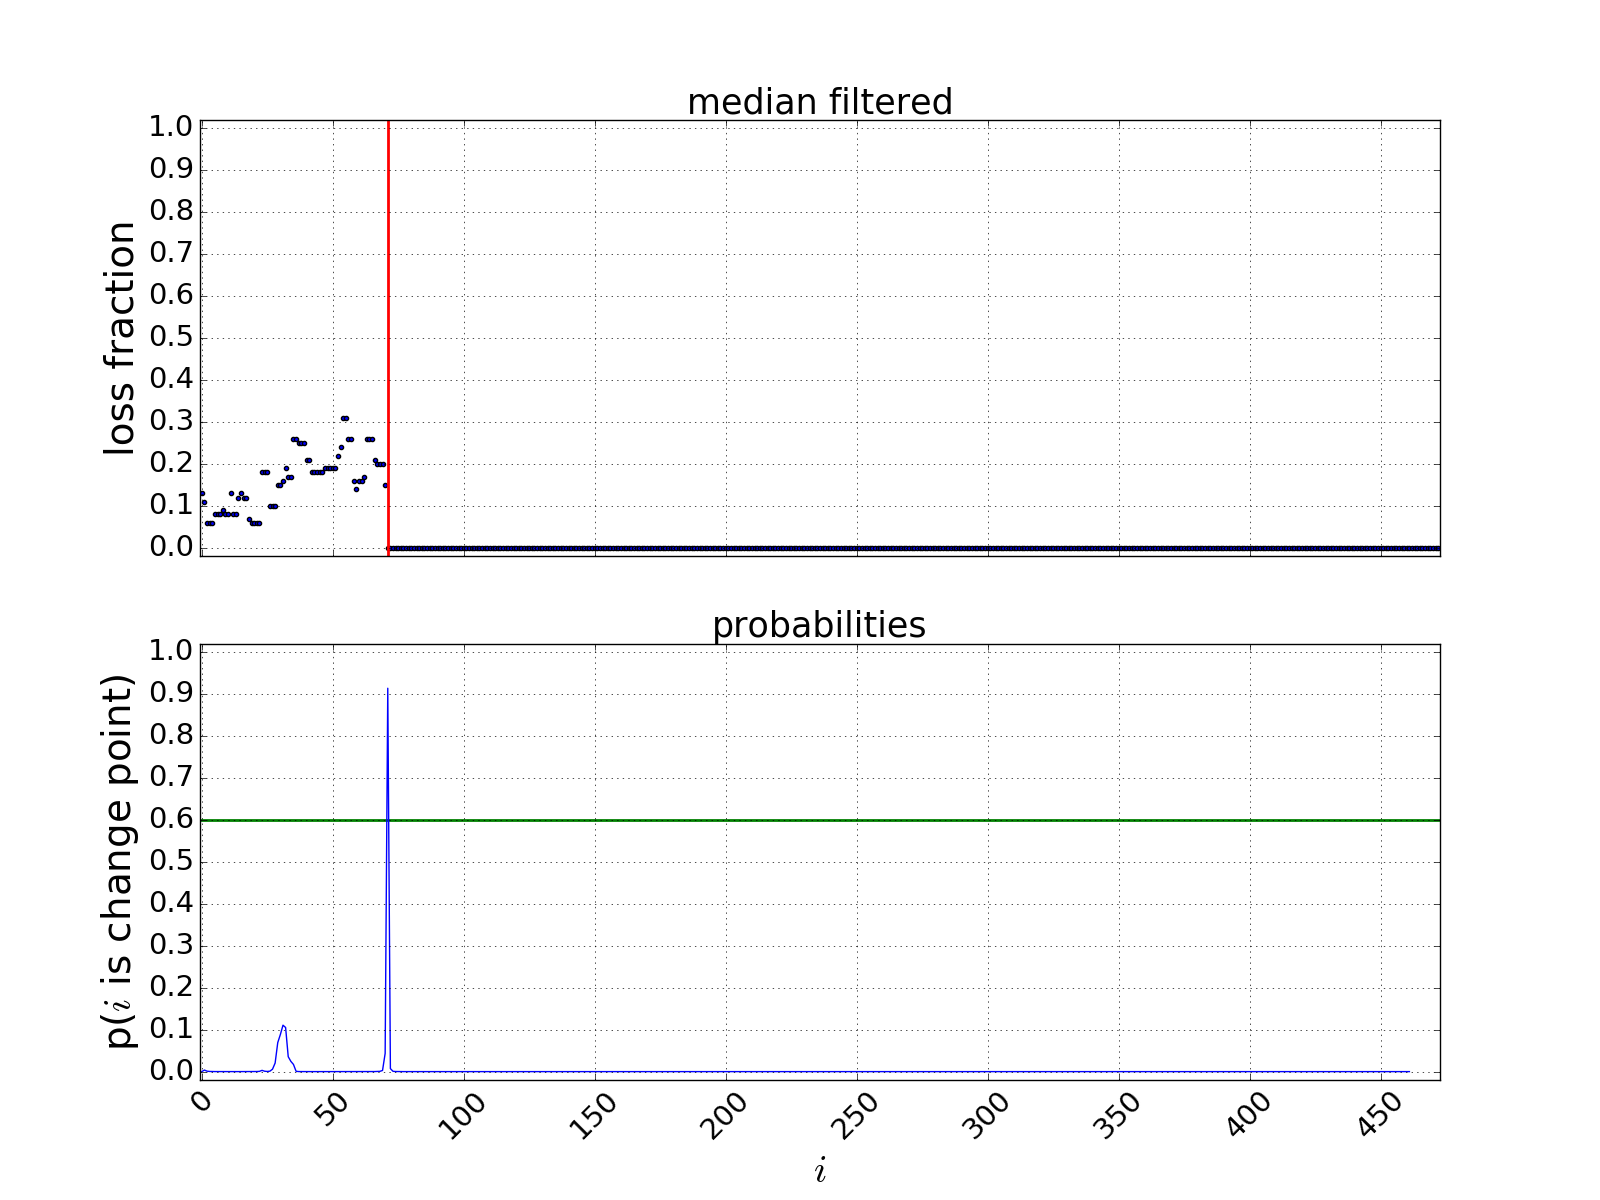
\includegraphics[width=\textwidth]{./figures/change_point_detection/bayesian_online/id305_serverSNEDTCPROB01_mac64:66:B3:A6:BB:80_dtstart2016-07-01_dtend2016-07-11.png}
            \caption{Online.}
        \end{subfigure}%
    }
    \caption{Bayesian Inference.}
\label{fig:bayesian_inference}
\end{figure}%

\section{Final Remarks}

Despite not being explicitly approached, it is possible to observe
through this chapter
that network measurements data has different patterns. Therefore,
the choice of the most appropriate set of algorithms and parameters
is one of the main difficulties of this project.
In Chapter~\ref{chap:methodology} this issue is discussed with more details.

The description of the parameters used in this
chapter can be found in appendix~\ref{}.
